%%%%%%%%%%%%%%%%%%%%%%%%%%%%%%%%%%%%%%%%%%%%%%%%%%%%%%%%%%%%%%%%%%%%%%
% LaTeX Template: Beamer arrows
%
% Source: http://www.texample.net/
% Feel free to distribute this template, but please keep the
% referal to TeXample.net.
% Date: Nov 2006
% 
%%%%%%%%%%%%%%%%%%%%%%%%%%%%%%%%%%%%%%%%%%%%%%%%%%%%%%%%%%%%%%%%%%%%%%
% How to use writeLaTeX: 
%
% You edit the source code here on the left, and the preview on the
% right shows you the result within a few seconds.
%
% Bookmark this page and share the URL with your co-authors. They can
% edit at the same time!
%
% You can upload figures, bibliographies, custom classes and
% styles using the files menu.
%
% If you're new to LaTeX, the wikibook is a great place to start:
% http://en.wikibooks.org/wiki/LaTeX
%
%%%%%%%%%%%%%%%%%%%%%%%%%%%%%%%%%%%%%%%%%%%%%%%%%%%%%%%%%%%%%%%%%%%%%%

\documentclass{beamer} %
\usetheme{CambridgeUS}

\usepackage[utf8]{inputenc}
\usefonttheme{professionalfonts}
\usepackage{times}
\usepackage{tikz}
\usepackage{amsmath}
\usepackage{verbatim}
\usepackage[francais]{babel}
\usetikzlibrary{arrows,shapes}
\usepackage{algorithm}
\usepackage{algorithmic}
\usepackage{bm}

\DeclareMathOperator*{\argmin}{arg\,min}

\author{Aris Tritas \and Laurent Cetinsoy}

\title{Know your customers}

\begin{document}
\maketitle
\begin{comment}
:Title: Beamer arrows
:Tags: Remember picture, Beamer, Physics & chemistry, Overlays
:Use page: 3

With PGF/TikZ version 1.09 and later, it is possible to draw paths between nodes across
different pictures. This is a useful feature for presentations with the
Beamer package. In this example I've combined the new PGF/TikZ's overlay feature
with Beamer overlays. Download the PDF version to see the result.

**Note.** This only works with PDFTeX, and you have to run PDFTeX twice.

| Author: Kjell Magne Fauske

\end{comment}


% For every picture that defines or uses external nodes, you'll have to
% apply the 'remember picture' style. To avoid some typing, we'll apply
% the style to all pictures.
\tikzstyle{every picture}+=[remember picture]

% By default all math in TikZ nodes are set in inline mode. Change this to
% displaystyle so that we don't get small fractions.
\everymath{\displaystyle}

\begin{frame}{Overview}

  \begin{figure}

    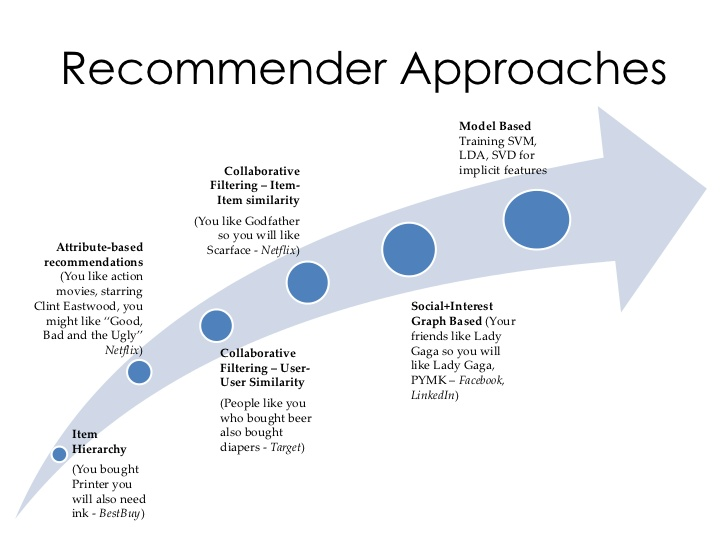
\includegraphics[width=10cm]{images/collaborative-filtering-and-recommender-systems-by-navisro-analytics-3-728}

  \end{figure}

\end{frame}

\begin{frame}{Customer affinity dataset}{Courtesy AlixML}
\begin{columns}
\begin{column}{0.5\textwidth}
\begin{itemize}
\item More than 2 millions of ratings of 3560 items from 93705 users
\item Sparsity:  $<1$\% of matrix filled
\item Split in 2.5M train \& 1.3M test examples
\item \#\{Ratings/Item\}: median=71, mean=712
\item \#\{Ratings/User\}: median=13, mean=28
\end{itemize}
\end{column}
\begin{column}{0.5\textwidth}  %%<--- here
    \begin{center}
    \begin{figure}
      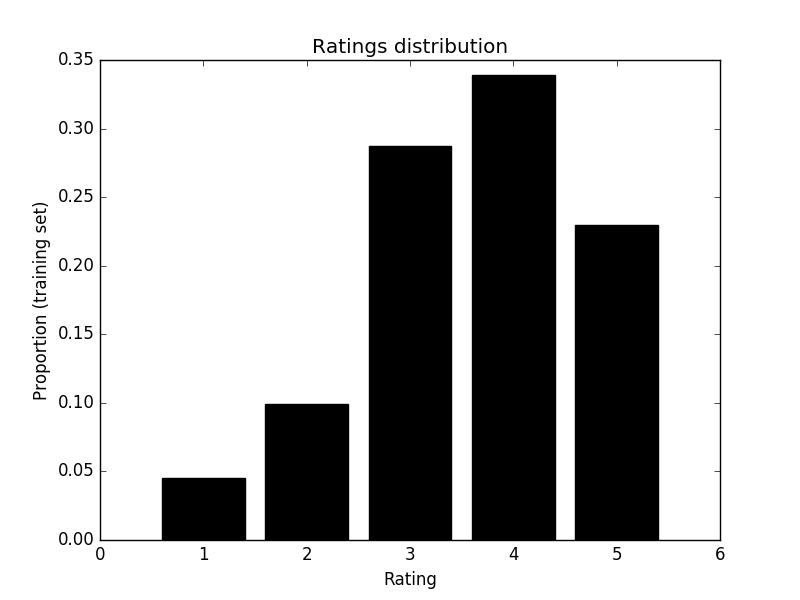
\includegraphics[height=5cm]{images/ratings.png}
    \end{figure}
     \end{center}
\end{column}
\end{columns}
\end{frame}


% Imaginons deux utilisateurs John-Bob et Alice.

%   \begin{equation*}
%   R_{1} = 
%   \begin{pmatrix}  
%       0 & 0 & 0 & 0 & 0 & \cdots & 0 \\
%   \end{pmatrix}
%   \end{equation*}

%   \begin{equation*}  
%   R_{2} = 
%   \begin{pmatrix}
 
%       0 & 0 & 1 & 0 & 0 & \cdots & 0 \\
%   \end{pmatrix}
%   \end{equation*}

%   \begin{equation*}  
%   R_{3} =    
%   \begin{pmatrix}  
%       0 & 0 & 1 & 0 & 0 & \cdots & 0 \\
%       0 & 4 & 1 & 0 & 0 & \cdots & 0 \\
%   \end{pmatrix}
%   \end{equation*}

%   \begin{equation*}
%   R_{4} = 
%     \begin{pmatrix}
%         0 & 3 & 1 & 3 & 0 & \cdots & 0 \\
%         0 & 4 & 1 & 0 & 0 & \cdots & 0 \\
%     \end{pmatrix}
%   \end{equation*}


% \begin{frame}{Collaborative filtering}{Formalisation}

%   \begin{equation*}
%   R_{n} = 
%   \begin{pmatrix}
  
%       0 & 3 & 1 & 3 & 0 & \cdots & 0 \\
%       0 & 4 & 1 & 0 & 0 & \cdots & 0 \\
      
%       \vdots & \vdots & \vdots & \vdots \\

%       4 & 2 & 1 & 3 & 0 & \cdots & 5 \\

%   \end{pmatrix}
% \end{equation*}      
% \end{frame}

\begin{frame}{Collaborative filtering}{Non negative factorization}

\begin{equation*}
	R = 
  \begin{pmatrix}  
      n_{11} & n_{12} & \cdots & n_{1i} \\
      n_{21} & n_{22} & \cdots & n_{2i} \\     
      \vdots & \vdots & \vdots & \vdots \\
      n_{u1} & n_{u2} & \cdots & n_{ui}
  \end{pmatrix}  =
  \overbrace{
   \begin{pmatrix}  
      n_{11} & \cdots & n_{1k} \\
      n_{21} & \cdots & n_{2k} \\      
      n_{31} & \cdots & n_{3k} \\
      \vdots & \vdots & \vdots \\
      n_{u1} & \cdots & n_{uk}
  \end{pmatrix}
  }^U
  \cdot
  \overbrace{
  \begin{pmatrix}  
      n_{11} & n_{12} & \cdots & n_{1i} \\
      n_{21} & n_{22} & \cdots & n_{2i} \\      
      \vdots & \vdots & \vdots & \vdots \\
      n_{k1} & n_{k2} & \cdots & n_{ki}
  \end{pmatrix}  
  }^{V^\mathrm{T}}
\end{equation*}

A new rating is computed as follows:
$$\tilde{r}_{ij} := u_i \cdot v_j^\mathrm{T} = \sum_{p=1}^{k} u_{ip}v_{pj} $$
      
\end{frame}

\begin{frame}{Collaborative filtering}{Non Negative Matrix Factorization}

  \begin{equation*}
      \begin{split}
       U^*, V^* =  \argmin_{U,V} & \frac{1}{2} ||R - UV^\mathrm{T}||^2 + \lambda \cdot \Omega(U, V) 
    \end{split}
  \end{equation*}
  
  $$R \in \mathbb{R}^{n \times m}, 
  			   U \in \mathbb{R}^{n \times k},
               V \in \mathbb{R}^{m \times k}$$
               	
  \onslide<2->{Usual regularization : $\Omega(U, V)  = ||U||^2 + ||V||^2$}


  \onslide<3->{Tikhonov  regularization: $\Omega(U, V)  = \sum_i \mathcal{J}(i) ||U_i||^2 + \sum_i \mathcal{I}(j)||V_i||^2$}


\end{frame}

\begin{frame}{NNMF}{Gradient Descent optimization}

Update rule using prediction error $e_{ij} = r_{ij} - \tilde{r}_{ij}$:
\begin{itemize}
\item $u_i \leftarrow u_i + \gamma \cdot (e_{ij} \cdot v_j - \lambda \cdot u_i)$
\item $v_j \leftarrow v_j + \gamma \cdot (e_{ij} \cdot u_i - \lambda \cdot v_j)$
\end{itemize}
avec $\gamma > 0$ le taux d'apprentissage, $\lambda > 0$ le coef. de régularisation

\vspace{20pt}
	
\end{frame}

\begin{frame}%[fragile]
    \frametitle{NNMF}
    \begin{algorithm}[H]
	\caption{ALS-WR}
	\label{disc1}
	\begin{algorithmic}[1]
	\WHILE{not happy}
    	\FOR{$i \in [n]$}
        \STATE $\hat{\bm{U}}_i \leftarrow \argmin_{\bm{U}} \sum_{j \in \mathcal{J}(i)} \big ( r_{ij} - \bm{U}\hat{V}_j^\mathrm{T} ) + \lambda \cdot \# \mathcal{J}(i) ||\bm{U} ||$ 
        \ENDFOR
        \FOR{$j \in [m]$}
        \STATE $\hat{\bm{V}}_j \leftarrow \argmin_{\bm{U}} \sum_{i \in \mathcal{I}(j)} \big ( r_{ij} - \hat{\bm{U}}_i{V}^\mathrm{T} ) + \lambda \cdot \# \mathcal{I}(j) ||\bm{V} ||$ 
        \STATE
        \ENDFOR
	  \ENDWHILE
	\end{algorithmic}
	\end{algorithm}
  \end{frame}


\begin{frame}{Results}{NMF}

$k = 15$

\begin{center}
    \begin{tabular}{|c|c|c|c|c|}
       \hline
       Model & ratings & k & lambda  & RMSE \\
       \hline
       GD  & 500k & 15 & 0.02 & 0.863 \\
	   GD & All & 15 & 0.02 &  0.951 \\
       ALS & 500k & 15 & 0.03 & 0.877 \\
	   ALS & All &  15  &  0.03 & 0.925 \\
       ALS & All & 30 & 0.03 &  0.923 \\
   	   ALS & All &  100  &  0.1 &   0.934 \\
       \hline
    \end{tabular}
  \end{center}

\end{frame}

\begin{frame}{Results}{Gradient descent}

$k = 15, \lambda = 0.02$
 \begin{center}
    \begin{tabular}{|c|c|c|c|}

       \hline
       Ratings & Left deletion & Righ deletion & RMSE \\
       \hline
       500k & 0 & 0 & 0.863 \\
       500k & 0 & 0.2 & 0.879\\

       All & 0 & 0 & 0.898 \\
       All & 0 & 0.2 & 0.911 \\      
       \hline
    \end{tabular}
  \end{center}
\end{frame}

\begin{frame}{NMF - Results}{ALS-WR}

NMF optimized with ALS-WR

$k = 15$

  \begin{center}
    \begin{tabular}{|c|c|c|c|}

       \hline
       Rating & Left deletion & right deletion & RMSE \\
       \hline
       500k & 0 & 0 & 0.877 \\
       500k & 0.2 & 0 & 0.8867 \\
       500k & 0.15 & 0.15 & 0.895 \\
       All & 0 & 0 &  \\
       All &  0  &  0.2 &   0.939 \\
       All* & 0  & 0 & RMSE = 0.934 \\
       \hline
    \end{tabular}
  \end{center}
  
  * $k = 30, \lambda = 0.03$

\end{frame}

\begin{frame}{Collaborative Filtering Networks}{[Salakhutdinov et al. 06]}
	
    \begin{figure}
    
%     	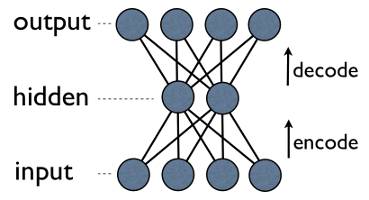
\includegraphics[height=5cm]{images/Auto-encodeur.png}
%     	\caption{Source: http://stats.stackexchange.com/a/117188}
    	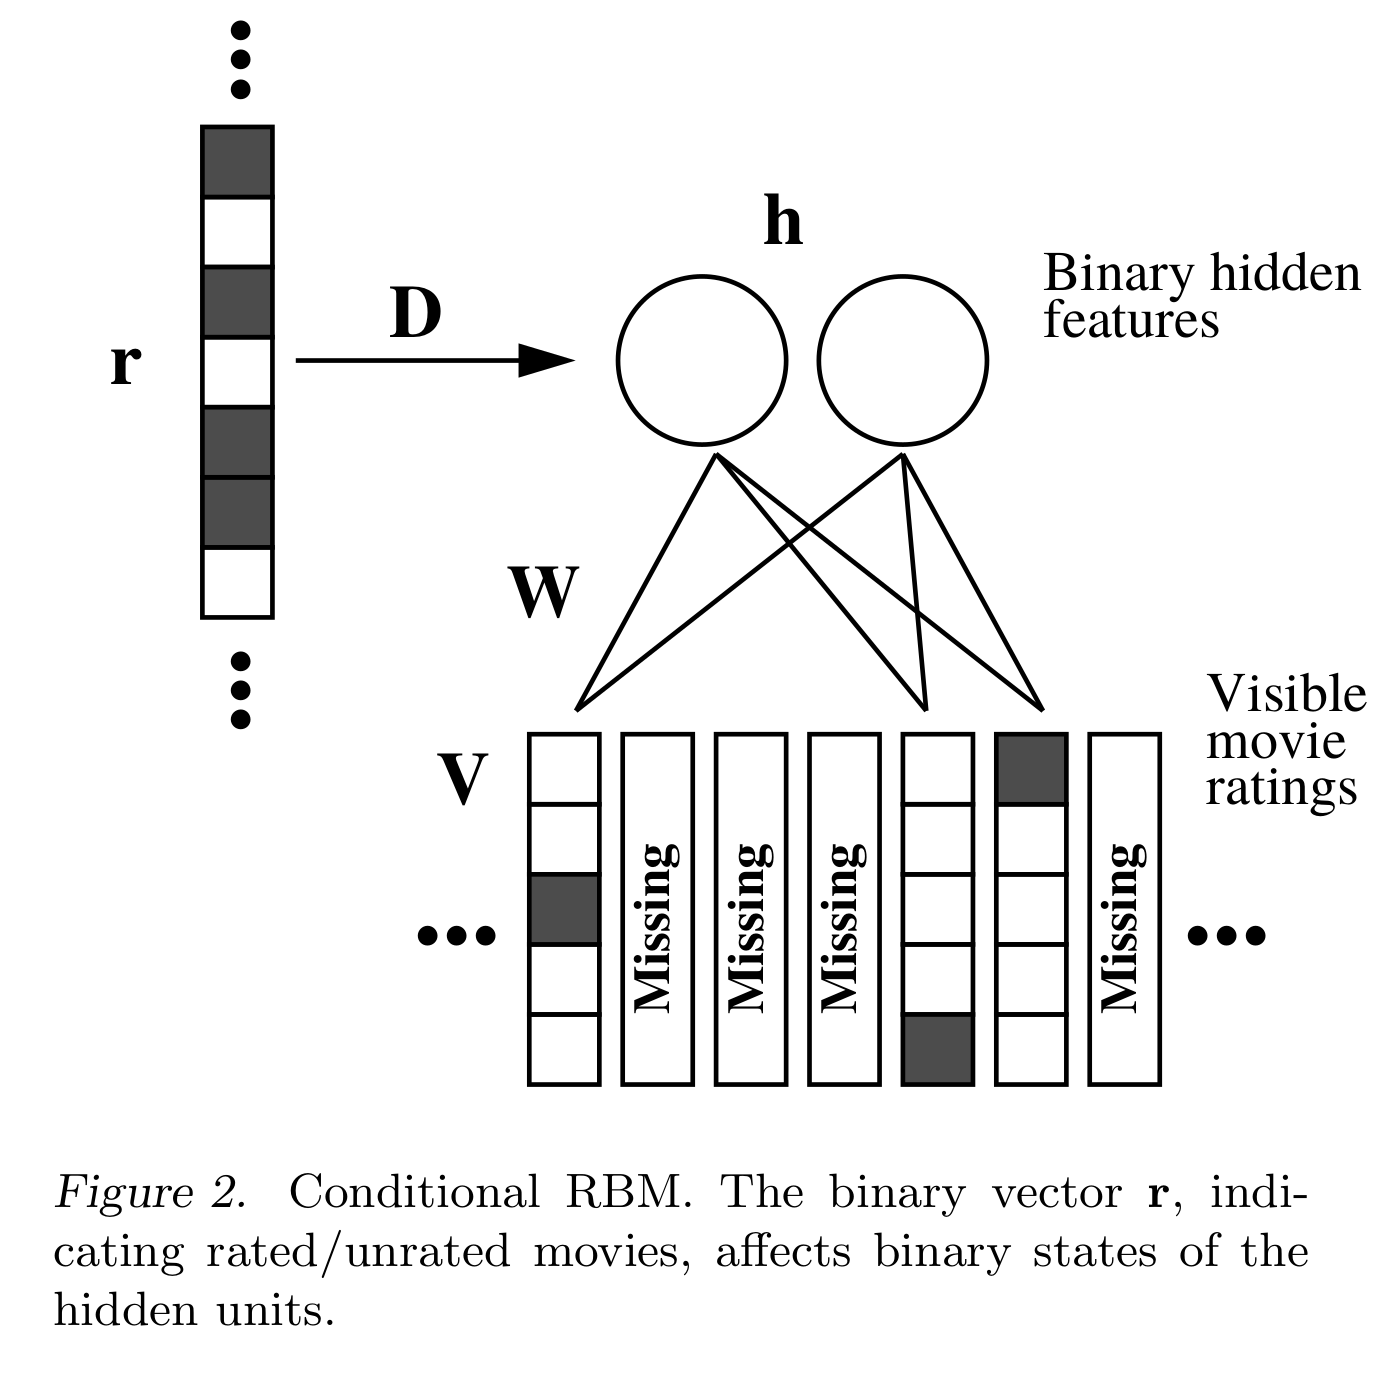
\includegraphics[width=0.5\textwidth]{images/conditional_rbm.png}
    	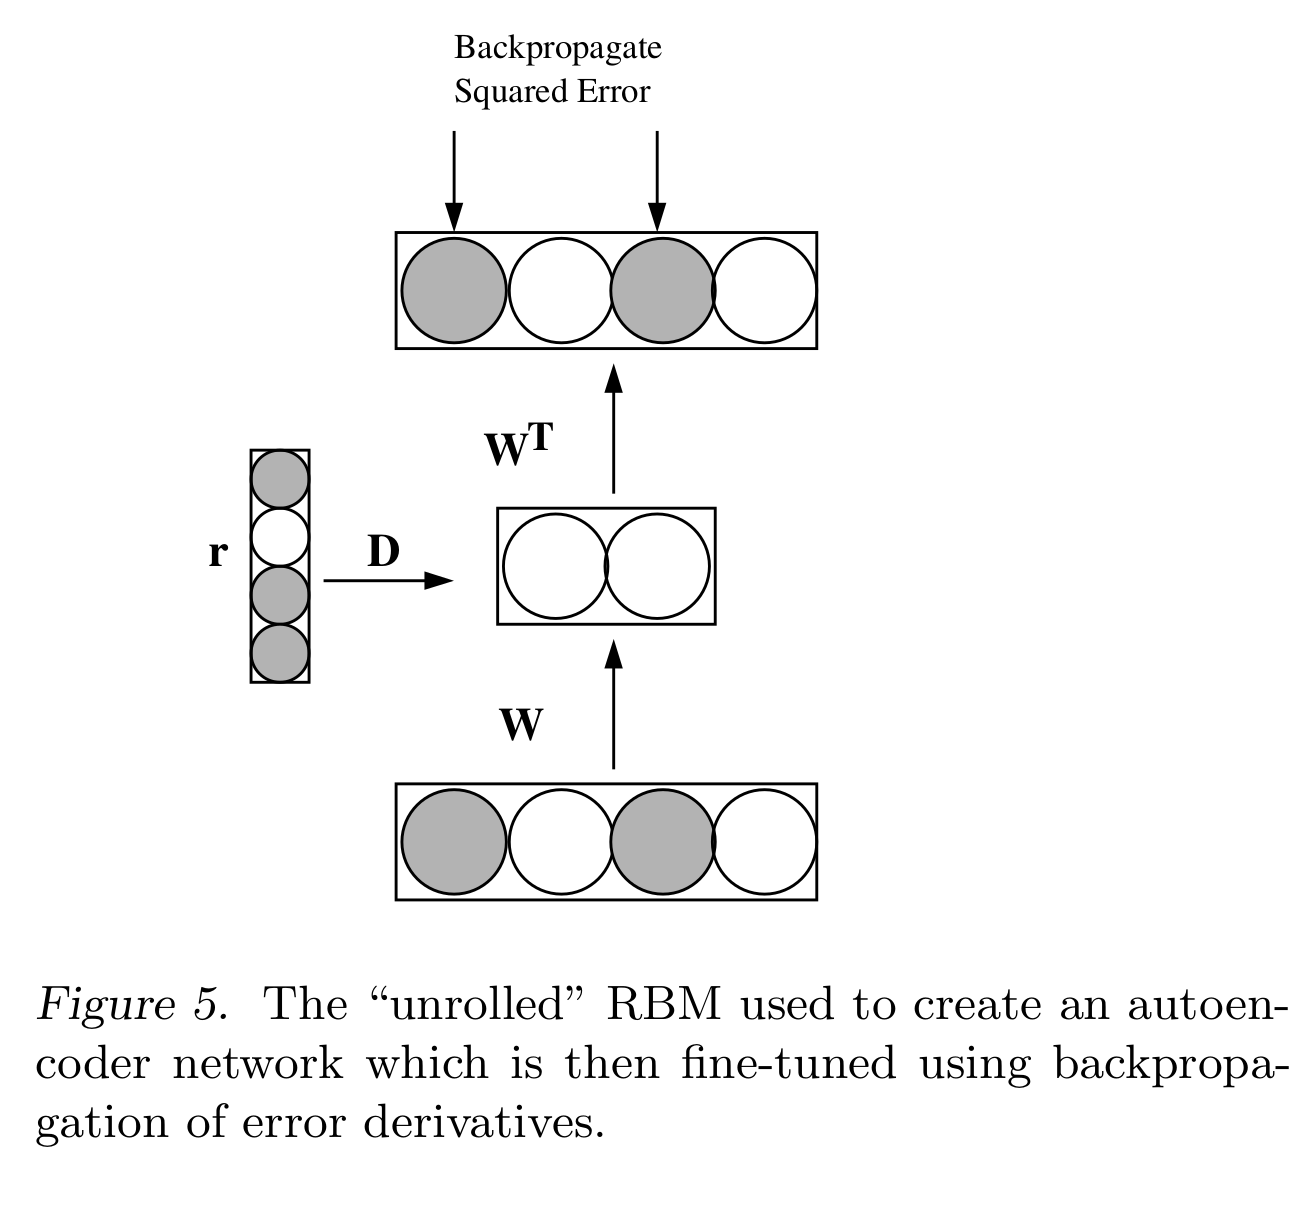
\includegraphics[width=0.5\textwidth]{images/unrolled_rbm.png}
    \end{figure}

\end{frame}

\begin{frame}{Hybrid collaborative Filtering with Autoencoders}{[Strub2016]}
\begin{equation*}
\begin{split}
  & f(\bm{x}) = \sigma(\bm{W_1 x+b_1}),\; g(\bm{y}) = \sigma(\bm{W_2 y+b_2} ) \; \;nn(\bm{x}) = g(f(\bm{x}))\\
  & \\
& L_{2, \alpha, \beta} = \alpha ( \sum_{j \in \mathcal{C}(\tilde{x})}) [ nn(\tilde{x}_j) - x_j ]^2 
+ \beta ( \sum_{j \notin \mathcal{C}(\tilde{x})} [nn(\tilde{x}_j) - x_j ]^2) \\
& \\
& \text{avec} \; \tilde{x} \in \mathbb{R}^N, W_1 \in \mathbb{R}^{K\times n}, W_1 \in \mathbb{R}^{n\times K}, b_1 \in \mathbb{R}^k, b_2 \in \mathbb{R}^N
\end{split}
\end{equation*}
\end{frame}

\begin{frame}{Hybrid collaborative Filtering with Autoencoders}{[Strub2016]}

    \begin{figure}
    
    	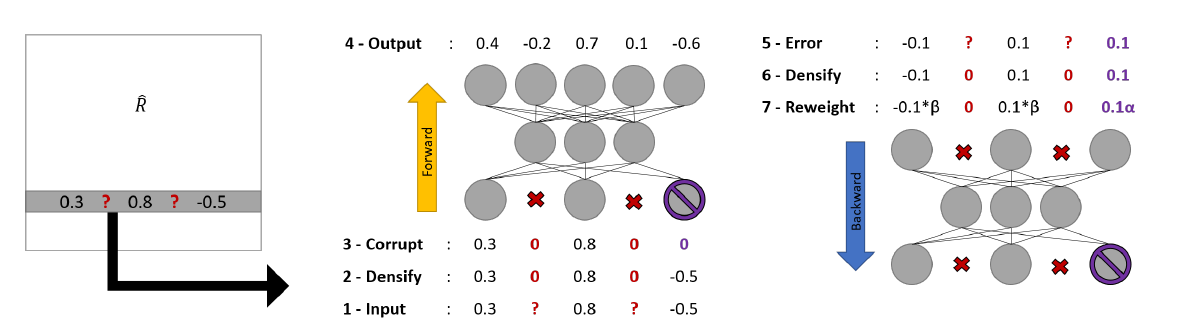
\includegraphics[width=12cm]{images/CF-with-AR-0.png}
    	\caption{On the forward pass the sparse input vector is densified and then corrupted. Before backpropagation, the error is reweighted and missing values are put to zero.}
    
    \end{figure}

\end{frame}

\begin{frame}{Injecting side-information}	

	\begin{figure}[h]
	  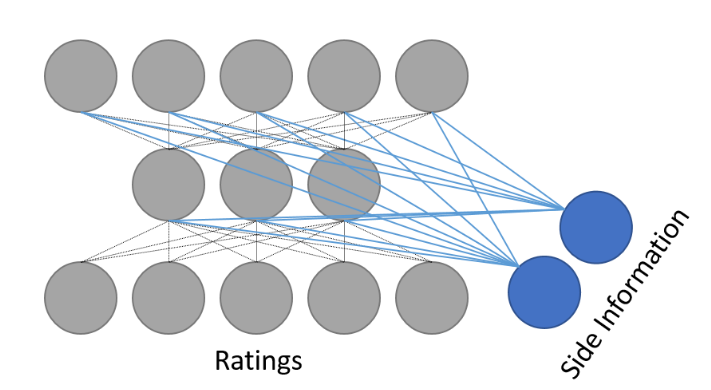
\includegraphics[width=10cm]{images/hybrid-cf-w-AE-2.png}
	\end{figure}

\end{frame}


\begin{frame}{Results}{Hybrid collaborative filtering with Autoencoders}

  \begin{center}
    \begin{tabular}{|c|c|c|c|c|}
    
       \hline
       Model & Rating & Left removal & right removal & RMSE \\
       \hline       
		AE Item Vector &  2M & 0 & 0 & 0.938 \\
        AE User Vector &  2M &  0  &  0 & 0.913 \\
   	    AE User Vector &  2M &  0  &  0.2 & 0.947 \\

       \hline
    \end{tabular}
  \end{center}
\end{frame}

\begin{frame}{Results}{Comparison between ALS and autoencoder networks.}
	\centering{
  \begin{figure}[t]
  \vspace*{-0.5cm}
    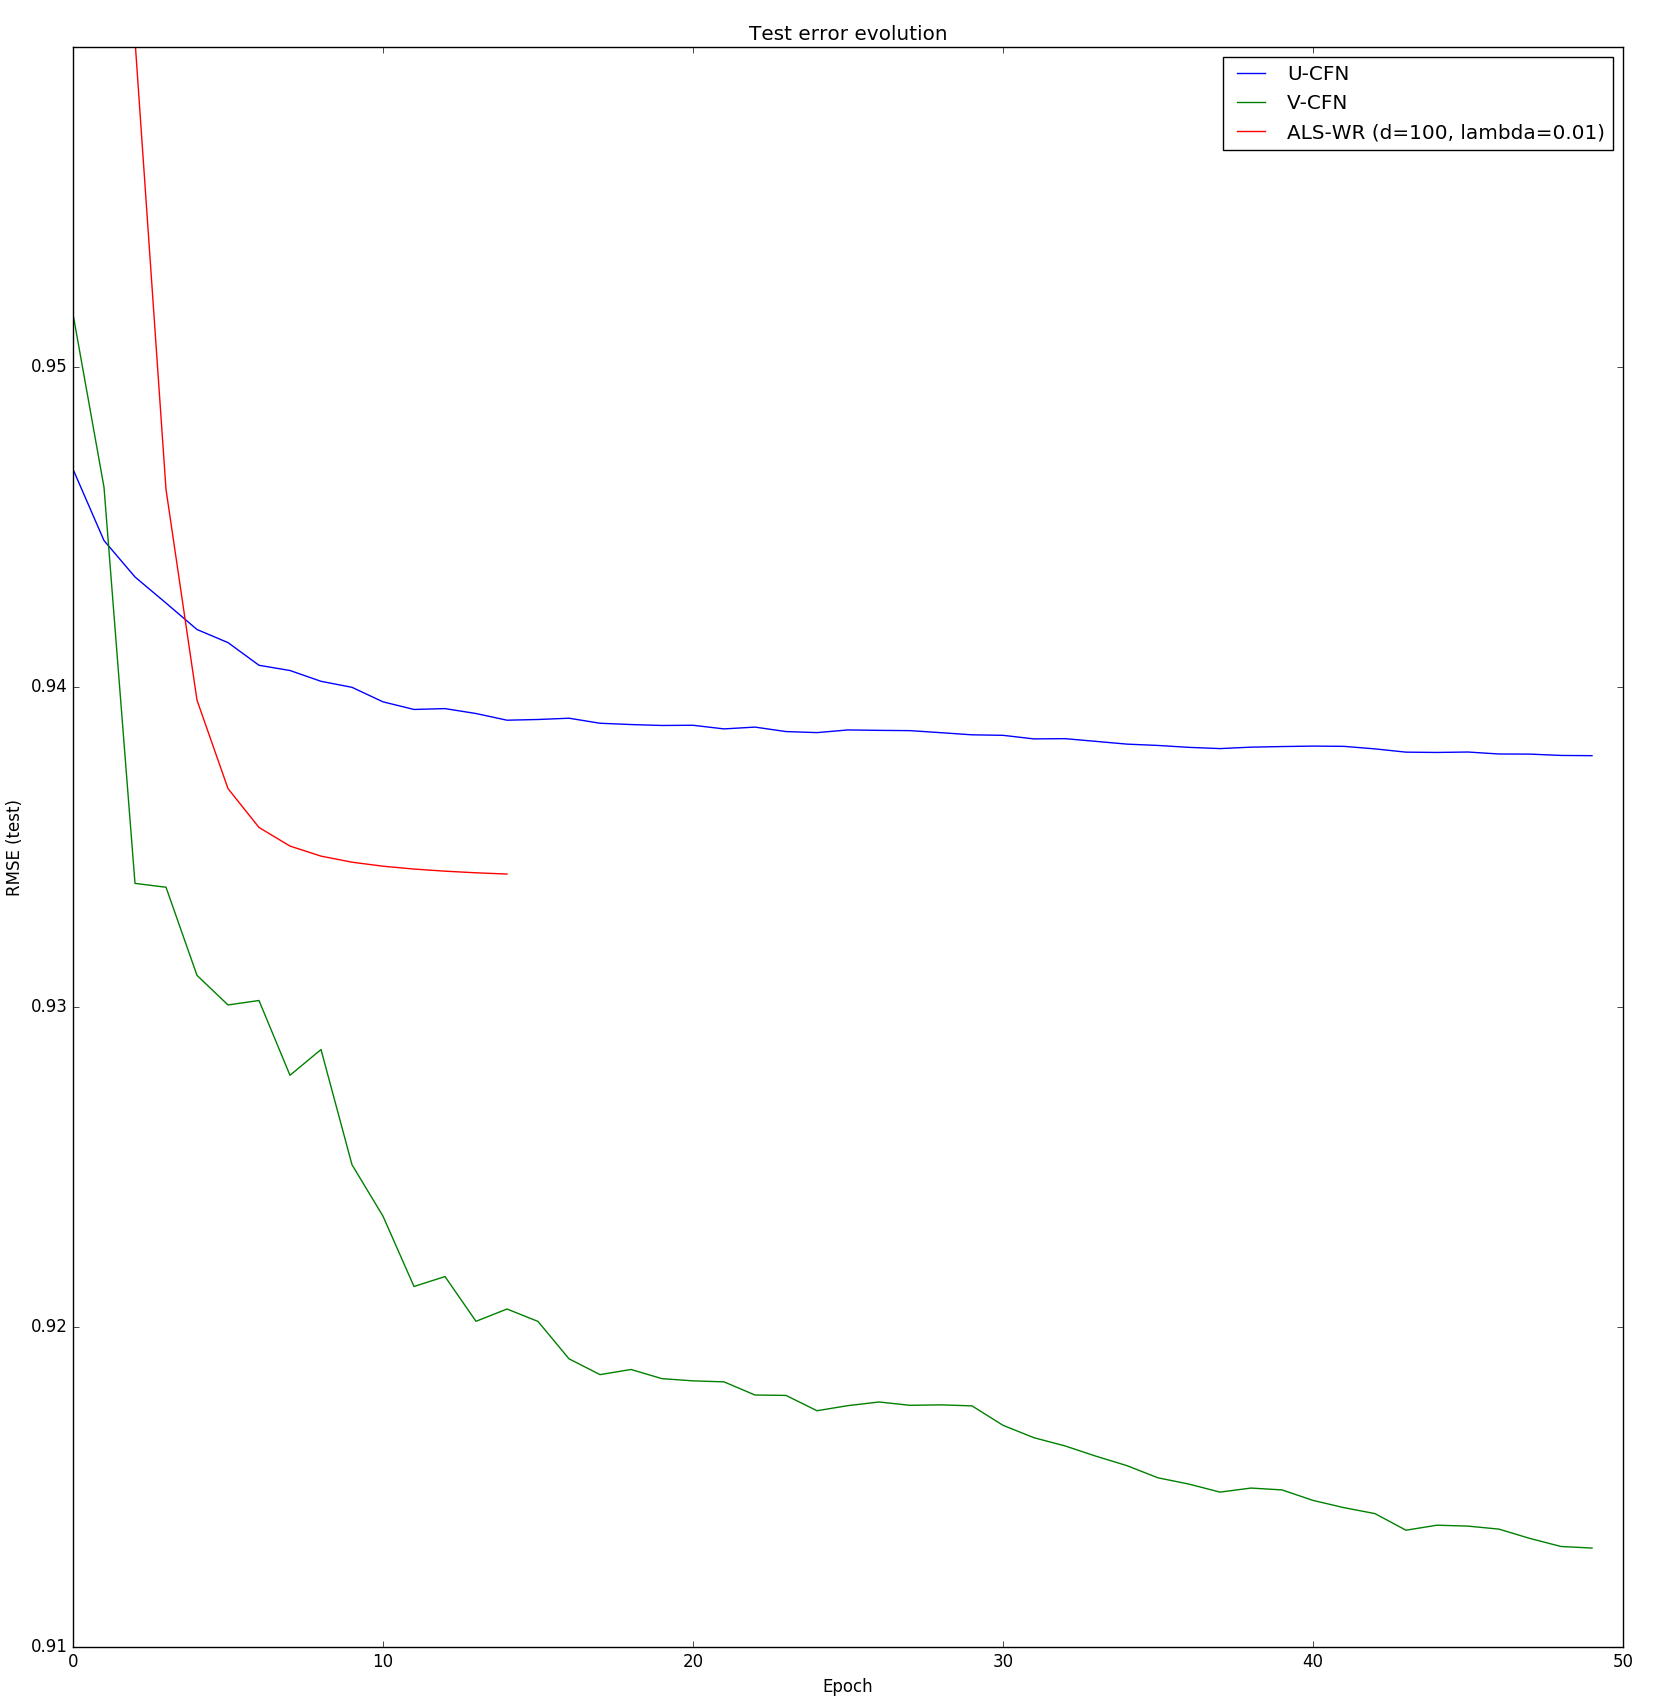
\includegraphics[height=6cm]{images/cfn.png}
	\caption{Test error evolution}
  \end{figure}
  }
\end{frame}


\begin{frame}{Conclusion, further work and ideas}

	\begin{itemize}
		\setlength\itemsep{2em}
        
        \item<1->{Add terms accounting for bias or temporal dynamics [Koren2009]}
        
        \item<2->{Further investigate dependency on succession}
       
		\item<3->{Hyperparameter tuning, better validation, effect of expert polling?} 
        %(regularization becomes an issue with deeper nets)
       
             	
	\end{itemize}

\end{frame}

\begin{frame}

	\begin{thebibliography}{10}
        
    \beamertemplatearticlebibitems
    
    \bibitem{Koren2009}{Y. Koren, R. Bell, C. Volinsky - Matrix factorization techniques for recommender systems. 2009 IEEE Computer Society}
       
    \bibitem{Strub2016}{F. Strub, J. Mary, R. Gaudel - Hybrid Collaborative Filtering with Auto-Encoders. Arxiv}

	\bibitem{Strub2016}{F. Strub, J. Mary, R. Gaudel - \url{https://github.com/fstrub95/Autoencoders_cf}}

	\bibitem{cfcode}{\url{https://github.com/lcetinsoy/collaborative-filtering}}
    
	\end{thebibliography}
\end{frame}

\end{document}